
%%%%

Very-high-end \sys-powered applications are expected to work around the clock, with a mean-time-to-recover of just a few seconds. \sys\ therefore needs to provide \emph{high availability (HA)}. 
Given that the underlying  data store is already highly available
and that client failures are tolerated by \sys's basic transaction processing protocol, 
\sys's HA solution only needs to address TM failures.
This is achieved via the primary-backup paradigm: during normal operation, a single \emph{primary} TM handles client requests, while a \emph{backup} TM runs in hot standby mode.
Upon detecting the primary's failure, the backup performs a \emph{failover} and becomes the new primary. 

The backup TM may falsely suspect that the primary has failed.
The resulting potential simultaneous operation of more than one TM creates challenges, which we discuss in 
Section~\ref{ssec:failover}. We address these in Section~\ref{ssec:basic} 
by adding synchronization to the transaction commit step. While such synchronization ensures correctness, it also introduces substantial overhead. We then optimize the solution in Section~\ref{ssec:opt}
to forgo synchronization during normal (failure-free) operation.

Our approach thus resembles 
many popular protocols, such as Multi-Paxos~\cite{Lamport:1998:PP:279227.279229} and its variants, which expedite normal mode operation as long as an agreed leader remains operational and unsuspected. However, by relying on shared persistent state in the underlying highly available data store, we obtain a simpler solution, eliminating the need to synchronize with a quorum in normal mode or to realign state during recovery.

%The latter is the actual implementation in \sys.  

\subsection{Failover and concurrent TMs} 
\label{ssec:failover}

The backup TM constantly monitors the primary's liveness.
Failure detection is timeout-based, namely, if the primary TM does not re-assert its existence within a configured period, it is deemed failed, and the backup starts acting as primary.  
Note that the primary and backup run independently on different machines, and the time it takes the primary to inform the backup that it is alive can be unpredictable due to network failures and processing delays, (e.g., garbage-collection stalls or long I/O operations). But in order to provide fast recovery, it is undesirable to set the timeout conservatively so as to ensure that a live primary is never detected as faulty.

We therefore have to account for the case that the backup performs failover and takes over the service while the primary is operational. 
Though such simultaneous operation of the two TMs is a necessary evil if one wants to ensure high availability, our design strives to reduce such overlap to a minimum. To this end, the primary TM actively checks if a backup has replaced it, and if so, ``commits suicide'', i.e., halts. However, it is still possible to have a (short) window between the failover and the primary's discovery of the existence of a new primary when two primary TMs are active. 

When a TM fails, all the transactions that began with it and did not commit (i.e., were not logged in the CT) are deemed aborted. 
%To prevent new transactions from seeing partial updates of transactions handled by the old TM, 
%The new TM needs to pick a starting logical clock time that exceeds all commit timestamps of transactions 
%that might still be committed by the old TM. 
However, this clear separation is challenged by the potential simultaneous existence of two TMs. For example, if the TM fails while a write it issued to the CT is still pending, the new TM may begin handling new transactions before the pending write takes effect. Thus, 
an old transaction may end up committing after the new TM has begun handling new ones. Unless handled carefully, this can cause a new transaction to see partial updates of old ones, as illustrated in Figure~\ref{fig:2TMs}.
To avoid this, we must ensure that once a new transaction obtains a read timestamp, the status of all transactions with smaller commit timestamps does not change.

A straightforward way to address the above challenge is via mutual exclusion, i.e., making sure that at most one TM commits operations at a time. However, this solution would entail synchronization upon each commit, not only at failover times, which would adversely affect performance. We therefore forgo this option.

\begin{figure}[t]
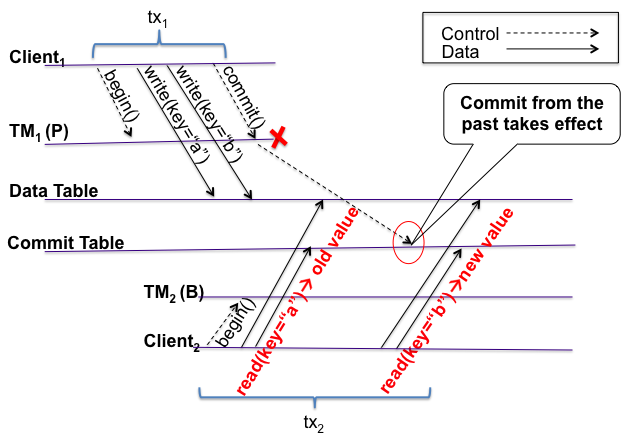
\includegraphics[width=\columnwidth]{omid_ha1.png}
\caption{{\bf The challenge with two concurrent TMs.} An old transaction, $tx_1$, commits while a new one $tx_2$ is processed, causing $tx_2$ to see an inconsistent snapshot. }
\label{fig:2TMs}
\end{figure}

\subsection{Basic HA algorithm}
\label{ssec:basic}  

Upon failover from $TM_1$ (the old primary) to $TM_2$ (the new one), we strive to ensure the following  properties:
\begin{description}
\item[P1] all timestamps assigned by $TM_2$ exceed all those assigned by $TM_1$; 
\item[P2] after a transaction $tx_2$ with read timestamp $ts2_r$ begins, no transaction $tx_1$ that will end up with a commit timestamp $ts1_c < ts2_r$ can update any additional data items (though it may still commit); and 
\item[P3] when a transaction reads a tentative update, 
it can determine whether this update will be committed with a timestamp smaller than its read timestamp or not.
\end{description}

Properties P1--P3 are sufficient for SI: P1 implies that commit timestamps continue to be totally ordered by commit time, P2 ensures that a transaction encounters every update that must be included in its snapshot, and P3 stipulates that the transaction can determine whether to return any read value.

To ensure the first two properties, the TMs publish the read timestamps they allot as part of initiating a transaction in a persistent shared object,   \emph{maxTS}. %(our implementation stores it in Apache Zookeeper~\cite{zookeeper}).
Before committing, the TM checks maxTS. If it finds a timestamp greater than its last committed one, it deduces that a new TM is active, aborts the transaction attempting to commit, and halts. 

In Figure~\ref{fig:2TMs} we saw  a scenario where the third property, P3, is violated--- when $tx_2$ reads key $a$ it cannot tell that $tx_1$, which wrote it, will end up committing with a smaller $ts1_c$ than $ts2_r$. 
This leads to an inconsistent snapshot at $tx_2$, as it sees the value of key $b$ written by $tx_1$.

To enforce P3, $tx_2$ cannot wait for $TM_1$, because the latter might have failed. Instead, we have $tx_2$ proactively abort $tx_1$, as illustrated in Figure~\ref{fig:invalidate}. 
%
More generally, when a read encounters a tentative update whose $txid$ is not present in the CT, it forces 
the transaction that wrote it to abort. We call this {\em invalidation}, and extend the CT's schema to include an \emph{invalid} field to this end.
Invalidation is performed via an atomic 
put-if-absent (supported by HBase's {\em checkAndMutate\/} API)
to the CT, which adds a record marking that $tx_1$ has  
``invalid'' status.  
The use of an atomic put-if-absent achieves \emph{consensus} regarding the state of the transaction.

Commits, in turn, read the CT after adding the commit record in order to check whether an invalidation record also exists, and if so, halt without returning a commit response to the client.  
In addition, every read of a tentative update checks its invalid field in the CT, and ignores the commit record if the transaction has been  invalidated.

\begin{figure}[t]
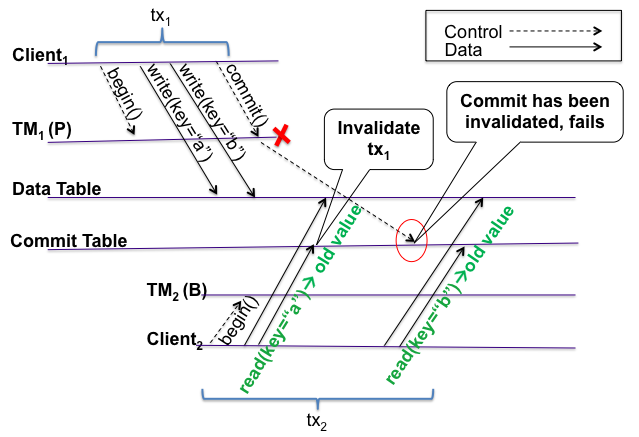
\includegraphics[width=\columnwidth]{omid_ha2.png}
\caption{{\bf Addressing the challenge of two concurrent TMs.} The old transaction is invalidated by the new one and therefore cannot commit.}
\label{fig:invalidate}
\end{figure}

While this solution satisfies the three required properties, it also induces a large number of synchronization steps:
(i) writing allotted read timestamps to maxTS to ensure P1; (ii) checking maxTS at commit time to ensure P2; and (iii)  
%using put-if-absent to invalidate a transaction in the shared CT every time a tentative update is encountered and 
checking  the CT for invalidation at the end of every commit to ensure P3. 
The next section presents an optimization that reduces the cost of synchronization.

\subsection{Synchronization-free normal operation}
\label{ssec:opt}

In order to eliminate the synchronization overhead most of the time, \sys's HA solution uses two mechanisms. 
First, to reduce the overheads  (i) and (ii) associated with timestamp synchronization, it 
allocates timestamp ranges in large chunks, called \emph{epochs}. 
That is, instead of incrementing maxTS by one timestamp at a time, the TM increments it by a certain \emph{range}, 
and is then free to allot timestamps in this range without further synchronization.
Second, to reduce  cost (iii) of checking for invalidations, 
it uses locally-checkable \emph{leases}, which are essentially locks that live for a limited time. As with locks, at most one TM may hold the lease at a given time (this requires the TMs' clocks to advance roughly at the same rate). 
\sys\ manages epochs and leases as shared objects in Zookeeper, and accesses them infrequently. 

Algorithm~\ref{alg:ha} summarizes the changes to support HA. On the TM side, 
{\sc CheckRenew} is called at the start of every commit and begin. 
It first  renews the lease every $\delta$ time, for some parameter $\delta$ (lines~\ref{l:lease-start}--\ref{l:lease-end}).
This parameter defines the tradeoff between synchronization frequency and recovery time:
the system can remain unavailable for up to $\delta$ time following a TM failure.
%
Since clocks may be loosely synchronized, \sys\ defines a {\em guard period\/} of $\delta' < \delta$, 
so that the lease must be renewed at least $\delta'$ time before it expires. 
%We assume the clock skew  between the TMs is smaller than this guard. 
The production default for $\delta'$ is $\delta/4$.
The primary TM fails itself (halts) if it cannot renew the lease prior to that time. 
From the clients' perspective, this is equivalent to a TM crash (line~\ref{l:lease-end}).
Second, {\sc CheckRenew} allocates a new epoch if needed (lines~\ref{l:epoch-start}--\ref{l:epoch-end}).

The backup (not shown in pseudocode) regularly checks the shared lease, and if it finds that it has expired, it immediately sets its clock to exceed maxTS,  
allocates a new epoch for itself (by increasing maxTS), and begins serving requests, \emph{without any special recovery procedure}.
Since the epoch claimed by a new TM always exceeds the one owned by the old one, Property P1 holds. 

Property P2 is enforced by having the TM (locally) check that its lease is valid before committing a transaction
(lines~\ref{l:lease-start}--\ref{l:lease-end}). 
Since at most one TM can hold the lease at a given time, and since the commit is initiated after all writes to items that are part of the transaction complete, Property P2  holds.

Nevertheless, the lease does not ensure Property P3, since the lease may expire while the commit record is in flight,
as in the scenario of Figures~\ref{fig:2TMs} and~\ref{fig:invalidate}. 
To this end, we use the invalidation mechanism described above. However, we limit its scope as follows: 
(1) A commit needs to check whether the transaction has been invalidated only if the TM's lease has expired.
This is done in the {\sc TMCheckInvalidate} function.
(2) A read needs to invalidate a transaction only if it pertains to an earlier epoch of a different TM. 
We extend client's {\sc GetTentativeValue} function to perform such invalidation 
in Algorithm~\ref{alg:ha} lines~\ref{l:invalidate-present},~\ref{l:invalidate-start}--\ref{l:invalidate-end}.
Note that a transaction reading a tentative update still checks its validity status regardless of the epoch, in order to avoid ``helping'' invalidated transactions complete their tentative updates. 
% Note that as long as a single TM is operational, \sys\  runs synchronization-free.





\begin{algorithm}[tb]
\begin{algorithmic}[1]
\algrestore{omid}
\begin{small}
\Procedure{CheckRenew}{} \\
 \Comment called by the TM at start of {\sc Begin} and {\sc Commit} 
\If{lease $<$ now + $\delta'$} \label{l:lease-start}
 \State renew lease for $\delta$ time \Comment atomic operation
 \If{failed} halt \EndIf 
\EndIf  \label{l:lease-end}
\If{Clock $=$ epoch}  \label{l:epoch-start}
\State epoch $\leftarrow$ Clock +  range
\State extend maxTS  from Clock  to epoch 
\If{failed} halt \EndIf 
\EndIf  \label{l:epoch-end}
\EndProcedure
%
\Statex
\Procedure{TMCheckInvalidate}{txid} \\
 \Comment called by the TM before {\sc Commit} returns
\If{lease $<$ now + $\delta'$}
 \If{$txid$ invalid in CT} halt \EndIf 
\EndIf
\EndProcedure
\Statex
%
\Procedure{GetTentativeValue(rec)}{} \\
\Comment replaces same function from Algorithm~\ref{fig:get-pseudocode}
 \State lookup rec.version in CT
 \If{present}
      \If{invalidated} return nil \EndIf 	\label{l:invalidate-present}
       \State update rec.commit \Comment helping
       \If{rec.commit $< ts_r$}  return rec.value \EndIf
\Else
\Comment new code -- check if need to invalidate
\If{rec.version $\in$ old epoch by an old TM} \label{l:invalidate-start}
 \State invalidate $t$ in CT \Comment  try to invalidate
 \If{failed}
	\State lookup rec.version in CT
	\If{invalidated} return nil \EndIf
       \State update rec.commit \Comment helping
       \If{rec.commit $< ts_r$}   \State return rec.value \EndIf
\Else \Comment invalidated
	\State return nil
\EndIf \label{l:invalidate-end}
\Else \Comment original code -- no invalidation
         \State  rec $ \leftarrow$ ds.get(\emph{key}, rec.version)
         \If{rec.commit$\not=$nil $\wedge$ rec.commit $< ts_r$}
		\State return rec.value \EndIf %\EndIf
\EndIf
\EndIf
\State return nil
\EndProcedure
\end{small}
\end{algorithmic}
\caption{\sys's HA algorithm.}
\label{alg:ha}
\end{algorithm}

% {\bf Client failover. }
Finally ,we note that on TM failover, some clients may still
 be communicating with the old TM. While the old TM may
end up committing some of their requests, a problem arises
if the client times out on the old TM before getting the
commit response, since the client might unnecessarily retry a committed transaction. 
To avoid this problem, a client that times out on its TM checks the CT for the status of its transaction
before connecting to a new TM. If the status is still undetermined, the client tries to invalidate the  CT entry, thus either forcing the
transaction to abort or learning that it was committed (in case the invalidation fails). 
